\chapter{Fundamentals}
\section{Introduction}
This chapter dives into several exciting concepts that power this project. We'll begin by exploring cloud computing, its various service offerings, and the available options in this domain. Next, we'll delve into DevOps principles and the tools that empower its implementation. Finally, we'll unveil the specific tools chosen for this project and the reasoning behind their selection.

\section{Cloud Computing}
\paragraph*{Definition:}
Cloud computing is the on-demand availability of computer system resources, especially data storage and computing power, without direct active management by the user. A simple way to describe the Cloud is its multiple data centers available to many users over the Internet.
\par
\noindent
Cloud computing services are offered by various providers, with Amazon Web Services, Microsoft Azure, and Google Cloud Platform being some of the major players in the field.
\subsection*{Comparative study between cloud providers}
So it makes sense to compare the three major cloud providers to see which one is the best for our project.
\subsubsection*{strengths of the three major cloud providers \cite{webArticle1}}
\begin{itemize}
    \item \textbf{Amazon Web Services (AWS):} AWS has had almost a 7-year head-start and vastly more offerings at present than other competitors. With that head start, the available talent pool is larger, meaning that more people know AWS.
    \item \textbf{Microsoft Azure:} Azure provides a pretty compelling transition path to the cloud, also Microsoft has a large number of enterprise customers, and many of them are already using Microsoft products. This makes it easier for them to use Azure.
    \item \textbf{Google Cloud Platform (GCP):} Google just happens to originated one of the most popular container orchestration systems, that being Kubernetes. and with that, it has been able to leverage that reputation to attract customers to its cloud platform.
\end{itemize}
\subsubsection*{Weaknesses of the three major cloud providers \cite{webArticle1}}
\begin{itemize}
    \item \textbf{Amazon Web Services (AWS):} With its vast growth Amazon (the company that owns AWS) has become a direct rival to many retailers, and that has led to some customers looking for alternatives.
    \item \textbf{Microsoft Azure:} For the past decade or so, open-source software has found great acceptance, both on-prem and in the cloud, largely due to organizations seeking alternatives to commercial software vendors like Microsoft.
    \item \textbf{Google Cloud Platform (GCP):} Google has a reputation for killing off products that don't meet its expectations, and that has led to some customers being wary of using Google Cloud Platform.
\end{itemize}
\subsection*{Verdict}
since this project is about transitioning to the cloud, and the fact that the company Adactim has a golden partnership with Microsoft, we will be using Microsoft Azure as our cloud provider.

\section{Cloud Computing Services}
\paragraph*{Definition:} Cloud computing services are a broad set of services that are delivered over the internet. These services are divided into three main categories: Infrastructure as a Service (IaaS), Platform as a Service (PaaS), and Software as a Service (SaaS).
\subsection*{IaaS}
\noindent
\textbf{Definition:} IaaS provides virtualized computing resources that require the developer to manage the infrastructure, including the network, servers, and operating systems. and with this comes great flexibility and scalability.
\noindent \\
\textbf{Offered Services:} Azure offers a wide range of IaaS services, including virtual machines, storage, and networking. With this, we can simulate the on-premises infrastructure in the cloud with minimal changes.
\subsection*{PaaS}
\noindent
\textbf{Definition:} PaaS provides a platform allowing developers to build, run, and manage applications without the complexity of building and maintaining the infrastructure. This allows developers to focus on the application itself.
\noindent \\
\textbf{Offered Services:} Some of the PaaS services offered by Azure include Azure App Service and Azure Functions. and these services have built-in deployment strategies that can be selected.
\subsection*{SaaS}
\noindent
\textbf{Definition:} SaaS is a software distribution model in which applications are hosted by a third-party provider so developers don't have to install, maintain, or update the software.
\noindent \\
\textbf{Offered Services:} Azure offers a wide range of SaaS services, including Office 365, Dynamics 365, and many more. Unfortunately, these services are not relevant to us since we cannot use them to host our application.
\subsection*{Verdict}
After this brief overview of the cloud computing services, we can conclude that the IaaS and PaaS services are the most relevant to us, so I will implement the deployment plan using both of them and choose the most suitable one.

\section{Introduction to DevOps\cite{webArticle0}}
The goal of DevOps is to increase an organization's speed when it comes to delivering applications and services. Many companies have successfully implemented DevOps to enhance their user experience including Amazon, Netflix, etc.
DevOps streamlines the application deployment process. Following each code contribution (commit) to a designated branch, DevOps automates the necessary tasks to ensure the appropriate deployment occurs while ensuring the appropriate testing is completed.
\subsection{Devops lifecycle}
DevOps lifecycle is the methodology where professional development teams come together to bring products to market more efficiently and quickly. The structure of the DevOps lifecycle consists of Plan, Code, Building, Test, Releasing, Deploying, Operating,  and Monitoring.

\begin{figure}[htpb]
    \centering
    \frame{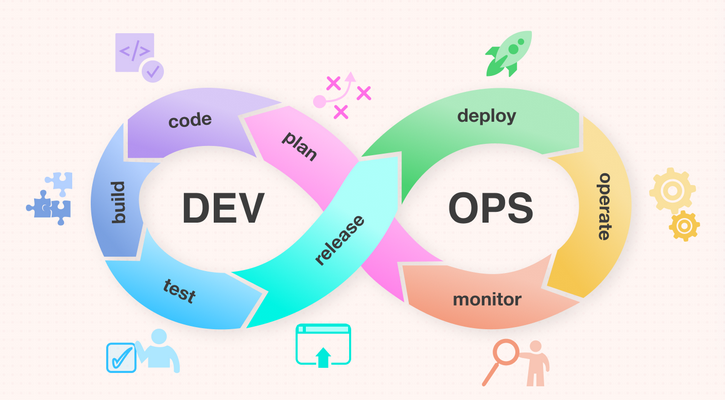
\includegraphics[width=0.8\columnwidth]{devop_lifecycle.png}}
    \caption{DevOps lifecycle}
    \label{fig:devops_lifecycle}
\end{figure}

\begin{itemize}
    \item \textbf{Plan:} gathering the opinions of end-users by professionals in this level of the DevOps lifecycle.
    \item \textbf{Code:} This is where the development team writes the code for the project.
    \item \textbf{Build:} This is where the development team compiles the code into a common code source.
    \item \textbf{Test:} Various sorts of tests are done such as user acceptability testing, safety testing, speed testing, and many more.
    \item \textbf{Release:} At this level, everything is ready to be deployed in the production environment.
    \item \textbf{Deploy:} In this level, Infrastructure-as-Code assists in creating the operational infrastructure and subsequently publishes the build.
    \item \textbf{Operate:} At this level, the available version is ready for users to use. Here, the department looks after the server configuration.
    \item \textbf{Monitor:} The observation is done at this level that depends on the data which is gathered from consumer behavior.
\end{itemize}

\subsection{Implementation of DevOps}
There are multiple ways to implement the DevOps methodology into a project:
\begin{itemize}
    \item \textbf{Leveraging Cloud-Based DevOps Solutions:}     Cloud providers like AWS, Azure, and GCP offer comprehensive DevOps platforms that integrate seamlessly with their respective cloud environments. These platforms provide pre-built tools for infrastructure provisioning, configuration management, CI/CD pipelines, and monitoring.
    \item \textbf{Using Open-source DevOps Tools:}DevOps tools like Jenkins, GitLab, Ansible, and Terraform provide the necessary automation and orchestration capabilities to streamline the development and deployment process. These tools can be integrated to create a customized DevOps pipeline tailored to the project's specific requirements.
\end{itemize}
Given that our web application resides in the cloud, leveraging a cloud-based DevOps solution offered by your chosen Cloud Service Provider (CSP) becomes an ideal approach. Here's why:
\begin{itemize}
    \item \textbf{Seamless Integration:} Cloud-based DevOps solutions integrate seamlessly with the underlying cloud infrastructure, offering pre-configured tools and services specifically designed for that environment. This translates to faster setup, easier management, and optimized performance for your cloud-hosted project.
    \item \textbf{Scalability and Elasticity:} Cloud-based solutions are inherently scalable and elastic. They can automatically adjust resources based on your project's demands, ensuring efficient resource utilization and cost optimization.
    \item \textbf{Managed Services:} Many cloud providers offer managed DevOps services that take care of infrastructure management, patching, and security updates. This frees up your team to focus on core development tasks.
\end{itemize}

\section{Description of available tools}

\subsection{Terraform}

\begin{figure}[htpb]
    \centering
    \frame{
\includegraphics[width=0.5\columnwidth]{Terraform.png}}
    \caption{Terraform}
    \label{fig:terraform}
\end{figure}

\textbf{Definition:} Imagine building your software on a foundation pre-designed with specific instructions, rather than individually placing each brick. This is the essence of Terraform, an open-source IaC tool. It allows you to define the infrastructure your application needs using a simple language, similar to writing instructions. This simplifies managing resources across different environments (cloud-based or on-premises) with consistent configurations, ensuring everything is built according to your specifications.
\par
\textbf{Alternatives:}
\begin{itemize}
    \item \textbf{Azure Resource Manager (ARM) templates:} These templates are native to Azure, offering familiarity and direct management within the platform. However, they require more technical knowledge and lack the flexibility and reliability of IaC tools like Terraform.
    \item \textbf{Bicep} Think of Bicep as a specialized architect fluent in Azure, Microsoft's cloud platform. It speaks Azure's language directly, making it easier to design and manage resources within that specific environment. However, since its expertise is limited to Azure it does not have the community support offered by an open-source project like Terraform.
\end{itemize}
By understanding these factors, we can make the informed decision that the IaC tool that best suits our requirements is Terraform.
\subsection{Azure DevOps}

\begin{figure}[htpb]
    \centering
    \frame{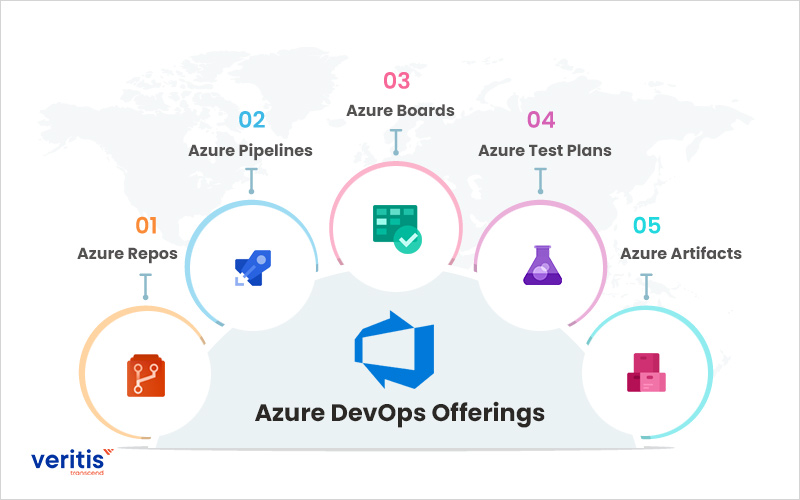
\includegraphics[width=0.5\columnwidth]{azure-devops-offerings.jpg}}
    \caption{Azure DevOps}
    \label{fig:Azure_DevOps}
\end{figure}

\textbf{Definition:} This platform acts as a comprehensive toolkit for software teams, offering various features to manage the entire development lifecycle efficiently.
\par
\textbf{Features:}
\begin{itemize}
    \item \textbf{Azure Repos:} This feature keeps your code organized and secure, just like a well-structured library holding all your project versions. It can use either Git or Team Foundation Version Control (TFVC) to manage your code.
    \item \textbf{Azure Pipelines:}  This service automates tasks like compiling code, running tests, and deploying new versions, saving time and minimizing errors.
    \item \textbf{Azure Boards:} Planning and tracking progress becomes transparent with this feature. It provides Kanban boards visually displaying tasks, backlogs listing upcoming work, and sprint planning tools.
    \item \textbf{Azure Artifacts:} Sharing reusable components becomes effortless with this feature. Think of it as a shared storage space for code modules, containerized applications, and other resources your team can easily access and reuse across projects.
\end{itemize}

\section*{Conclusion}
In this chapter we have explored the fundamentals of cloud computing, DevOps principles, and the tools that empower its implementation. And with this we have the list of recourses that will be used: Azure , Azure Devops and terraform. Later on , in the next chapter we will dive into the analatycs of the existing infrastructure and the specification of our needs.
